\documentclass[tikz,border=6pt]{standalone}
\usepackage[T1]{fontenc}
\usepackage[utf8]{inputenc}
\usepackage{pgfplots}
\usepgfplotslibrary{groupplots}
\usetikzlibrary{calc}
\pgfplotsset{compat=1.18}
\begin{document}
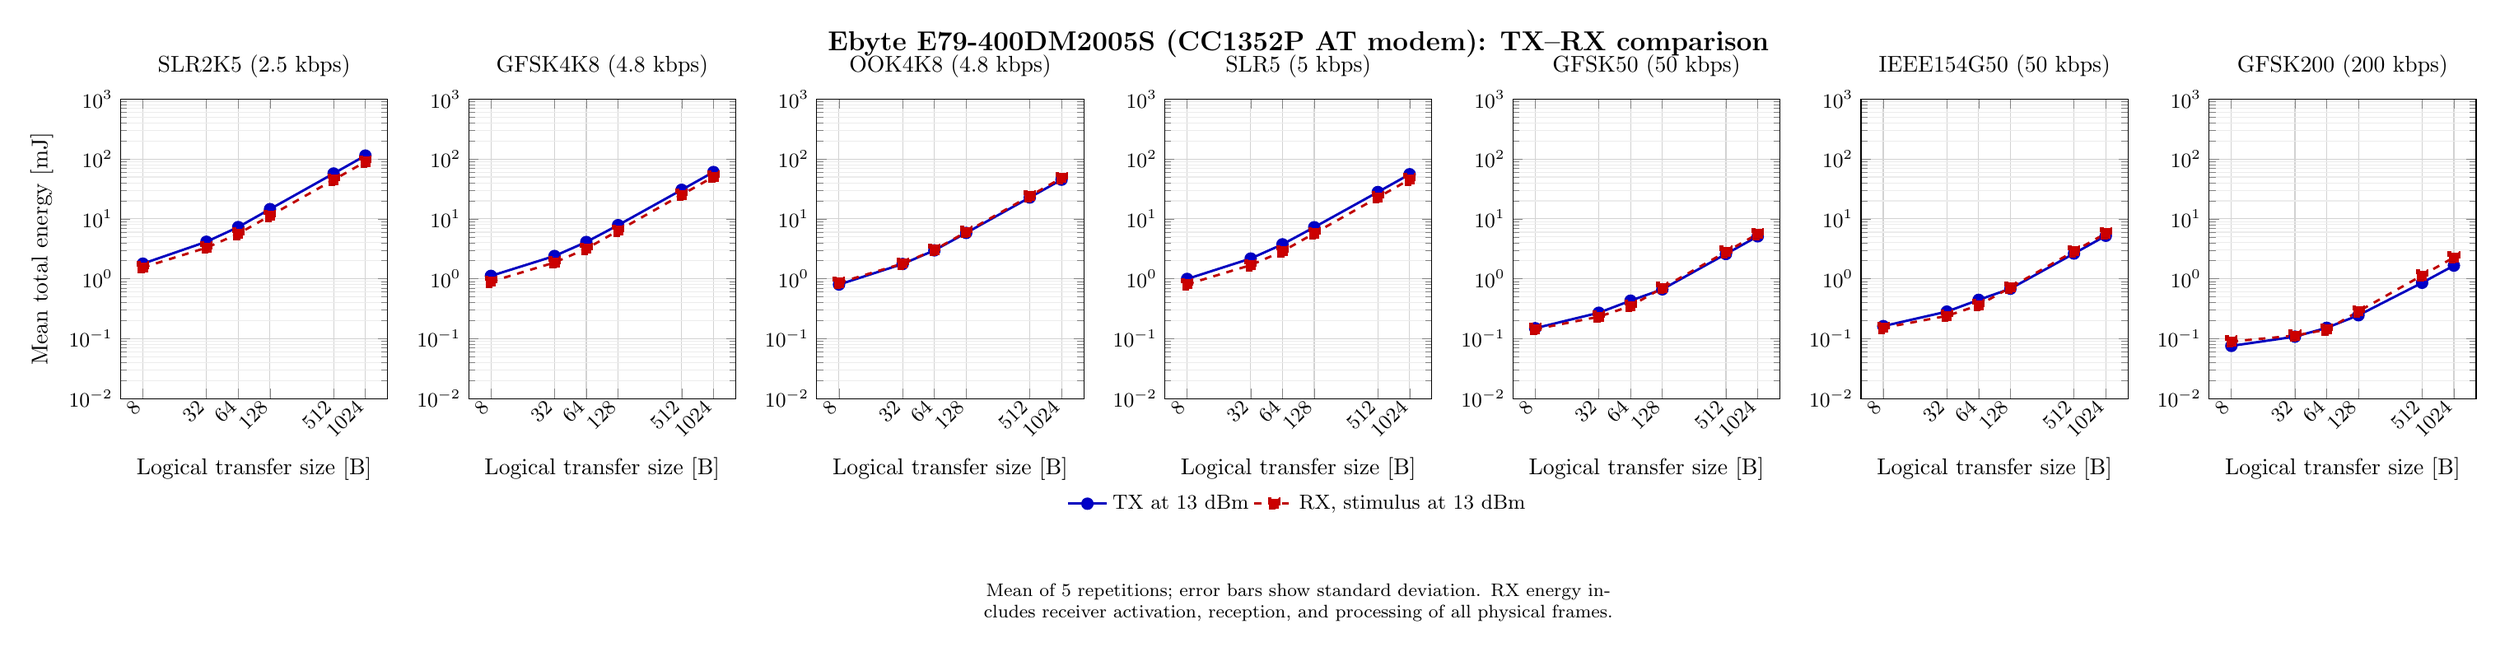
\begin{tikzpicture}
\begin{groupplot}[/pgf/number format/use comma,
  group style={group size=7 by 1, horizontal sep=1.25cm},
  width=5.7cm, height=6.2cm,
  xmode=log, log basis x={2}, ymode=log, log basis y={10},
  ymin=0.01, ymax=1000,
  xtick={8,32,64,128,512,1024}, xticklabels={8,32,64,128,512,1024},
  x tick label style={rotate=45, anchor=east, font=\small},
  y tick label style={font=\small},
  grid=both, minor grid style={gray!15}, major grid style={gray!35},
  xlabel={Logical transfer size [B]},
  every axis plot/.append style={line width=1.05pt},
  error bars/error bar style={line width=0.35pt},
  legend style={font=\small, draw=none, fill=none, at={(0.5,-0.29)},
    anchor=north, legend columns=-1},
]
\nextgroupplot[title={SLR2K5 (2.5 kbps)}, ylabel={Mean total energy [mJ]}]
\addplot+[color=blue!75!black, solid, mark=*, mark size=2.2pt,
  error bars/.cd, y dir=both, y explicit,
] coordinates {
  (8,1.78682554) +- (0,0.00193720275)
  (32,4.14961761) +- (0,0.00643593785)
  (64,7.29493148) +- (0,0.0126967254)
  (128,14.5605686) +- (0,0.0379098161)
  (512,57.2527543) +- (0,0.0602916345)
  (1024,114.028554) +- (0,0.117074788)
};
\addplot+[color=red!75!black, dashed, mark=square*, mark size=2.2pt,
  error bars/.cd, y dir=both, y explicit,
] coordinates {
  (8,1.54484922) +- (0,0.00210628524)
  (32,3.30214535) +- (0,0.00716936278)
  (64,5.6381009) +- (0,0.0103344026)
  (128,11.2741123) +- (0,0.0170795493)
  (512,44.9095583) +- (0,0.0691906586)
  (1024,89.7871744) +- (0,0.0952640524)
};
\nextgroupplot[title={GFSK4K8 (4.8 kbps)}]
\addplot+[color=blue!75!black, solid, mark=*, mark size=2.2pt,
  error bars/.cd, y dir=both, y explicit,
] coordinates {
  (8,1.11575312) +- (0,0.00299768886)
  (32,2.39937627) +- (0,0.00648337206)
  (64,4.10935177) +- (0,0.00687165253)
  (128,7.85627879) +- (0,0.024885918)
  (512,30.5631105) +- (0,0.0526300401)
  (1024,60.6147494) +- (0,0.113818251)
};
\addplot+[color=red!75!black, dashed, mark=square*, mark size=2.2pt,
  error bars/.cd, y dir=both, y explicit,
] coordinates {
  (8,0.894054962) +- (0,0.00205062849)
  (32,1.86754915) +- (0,0.0060153713)
  (64,3.17319687) +- (0,0.00636874861)
  (128,6.34233948) +- (0,0.0138302055)
  (512,25.2672042) +- (0,0.0435204954)
  (1024,50.4618265) +- (0,0.0439855681)
};
\nextgroupplot[title={OOK4K8 (4.8 kbps)}]
\addplot+[color=blue!75!black, solid, mark=*, mark size=2.2pt,
  error bars/.cd, y dir=both, y explicit,
] coordinates {
  (8,0.801347946) +- (0,0.00269755522)
  (32,1.76326219) +- (0,0.00670972562)
  (64,2.98277785) +- (0,0.00281687772)
  (128,5.83050029) +- (0,0.0116424233)
  (512,22.762573) +- (0,0.0211711607)
  (1024,45.2156346) +- (0,0.0618876963)
};
\addplot+[color=red!75!black, dashed, mark=square*, mark size=2.2pt,
  error bars/.cd, y dir=both, y explicit,
] coordinates {
  (8,0.85857959) +- (0,0.00260799118)
  (32,1.79230825) +- (0,0.00634443878)
  (64,3.03222321) +- (0,0.00496867964)
  (128,6.05517294) +- (0,0.0127428676)
  (512,24.0750147) +- (0,0.0582632667)
  (1024,48.0307046) +- (0,0.0611305901)
};
\nextgroupplot[title={SLR5 (5 kbps)}]
\addplot+[color=blue!75!black, solid, mark=*, mark size=2.2pt,
  error bars/.cd, y dir=both, y explicit,
] coordinates {
  (8,0.992945309) +- (0,0.0015784517)
  (32,2.17604681) +- (0,0.00314660668)
  (64,3.7570602) +- (0,0.00369477244)
  (128,7.25109863) +- (0,0.027072279)
  (512,28.0706404) +- (0,0.060897947)
  (1024,55.6383125) +- (0,0.119776105)
};
\addlegendentry{TX at 13 dBm}
\addplot+[color=red!75!black, dashed, mark=square*, mark size=2.2pt,
  error bars/.cd, y dir=both, y explicit,
] coordinates {
  (8,0.808907874) +- (0,0.001628945)
  (32,1.68977846) +- (0,0.00668059998)
  (64,2.86682007) +- (0,0.00525161075)
  (128,5.73793942) +- (0,0.0096134487)
  (512,22.8286715) +- (0,0.0296112196)
  (1024,45.535809) +- (0,0.0746059636)
};
\addlegendentry{RX, stimulus at 13 dBm}
\nextgroupplot[title={GFSK50 (50 kbps)}]
\addplot+[color=blue!75!black, solid, mark=*, mark size=2.2pt,
  error bars/.cd, y dir=both, y explicit,
] coordinates {
  (8,0.149257074) +- (0,0.000998008295)
  (32,0.270372655) +- (0,0.00110112891)
  (64,0.430289998) +- (0,0.00221702985)
  (128,0.666311061) +- (0,0.000866845194)
  (512,2.59209225) +- (0,0.0115005492)
  (1024,5.11540087) +- (0,0.00783537147)
};
\addplot+[color=red!75!black, dashed, mark=square*, mark size=2.2pt,
  error bars/.cd, y dir=both, y explicit,
] coordinates {
  (8,0.143588725) +- (0,0.000380378927)
  (32,0.231912272) +- (0,0.00182275501)
  (64,0.349205027) +- (0,0.00092766977)
  (128,0.702941404) +- (0,0.00221723551)
  (512,2.80486225) +- (0,0.00485655898)
  (1024,5.6061666) +- (0,0.00686623397)
};
\nextgroupplot[title={IEEE154G50 (50 kbps)}]
\addplot+[color=blue!75!black, solid, mark=*, mark size=2.2pt,
  error bars/.cd, y dir=both, y explicit,
] coordinates {
  (8,0.161736921) +- (0,0.000876658039)
  (32,0.282554274) +- (0,0.00196616361)
  (64,0.443979802) +- (0,0.00131216071)
  (128,0.682422789) +- (0,0.00221809947)
  (512,2.63993299) +- (0,0.0357372308)
  (1024,5.22479192) +- (0,0.010542337)
};
\addplot+[color=red!75!black, dashed, mark=square*, mark size=2.2pt,
  error bars/.cd, y dir=both, y explicit,
] coordinates {
  (8,0.151248005) +- (0,0.00157234453)
  (32,0.239683745) +- (0,0.00165309447)
  (64,0.359581931) +- (0,0.000909499216)
  (128,0.716879143) +- (0,0.00326322902)
  (512,2.87131949) +- (0,0.00350523924)
  (1024,5.72614902) +- (0,0.0146383721)
};
\nextgroupplot[title={GFSK200 (200 kbps)}]
\addplot+[color=blue!75!black, solid, mark=*, mark size=2.2pt,
  error bars/.cd, y dir=both, y explicit,
] coordinates {
  (8,0.0756527262) +- (0,0.000878431519)
  (32,0.10788161) +- (0,0.00118107306)
  (64,0.151540968) +- (0,0.00101543015)
  (128,0.245744313) +- (0,0.00107293936)
  (512,0.85730023) +- (0,0.0013454389)
  (1024,1.66032186) +- (0,0.0082014162)
};
\addplot+[color=red!75!black, dashed, mark=square*, mark size=2.2pt,
  error bars/.cd, y dir=both, y explicit,
] coordinates {
  (8,0.0894733247) +- (0,0.000776323572)
  (32,0.112356538) +- (0,0.00119579262)
  (64,0.141583569) +- (0,0.00101582445)
  (128,0.285475981) +- (0,0.00129695024)
  (512,1.13568622) +- (0,0.00178211566)
  (1024,2.27628632) +- (0,0.00421761454)
};
\end{groupplot}
\node[font=\bfseries\large] at ($(group c4r1.north)+(0,0.85cm)$)
  {Ebyte E79-400DM2005S (CC1352P AT modem): TX--RX comparison};
\node[font=\footnotesize, align=center, text width=18.5cm]
  at ($(group c4r1.south)+(0,-3.15cm)$)
  {Mean of 5 repetitions; error bars show standard deviation. RX energy includes receiver activation, reception, and processing of all physical frames.};
\end{tikzpicture}
\end{document}
